
\section{Analyse}

	
	\subsection{Le déroulement du jeu}


		\begin{figure}[h]
			\begin{center}
				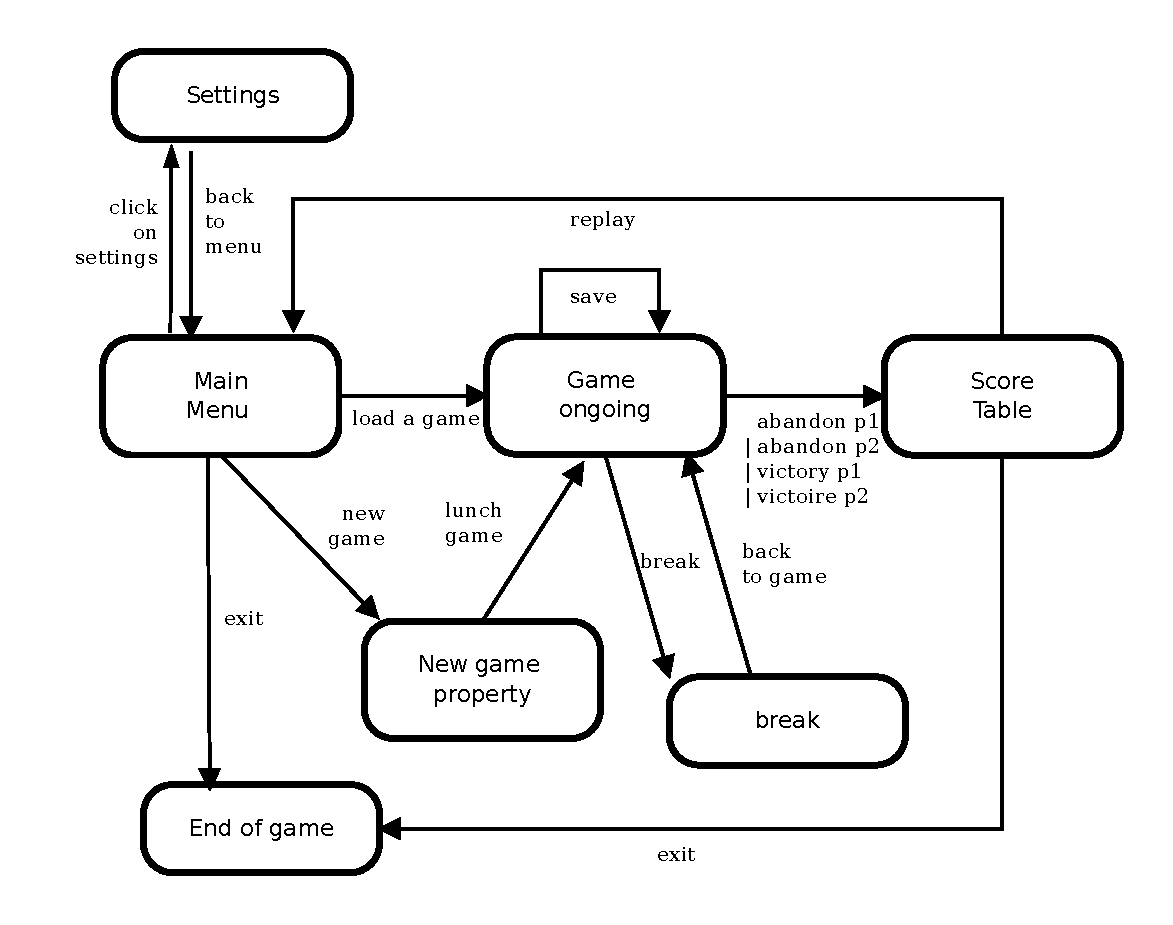
\includegraphics[width=0.7\textwidth]{figure/etat_transition_partie.pdf}
			\end{center}
			\caption{Diagrame d'états-transitions}
			\label{fig:transition_jeu}
		\end{figure}
	
		le diagramme d'état-transition présenté en FIGURE \ref{fig:transition_jeu} présente les différents état dans lequel le programme \emph{Bedbihan} peut se situer, il modélise ainsi les différentes phases du jeu.


		\subsection{Le lancement du jeu}

		Au lancement du jeu, l'utilisateur a le choix entre débuter une nouvelle partie et reprendre une partie préalablement sauvegardée. Le lancement d'une nouvelle partie implique le choix d'une taille de carte, ainsi que le choix d'un peuple pour chacun des joueurs. 

		Ceci est illustré par le diagramme d'utilisation présenté en FIGURE \ref{fig:use1}.

		\begin{figure}
			\begin{center}
				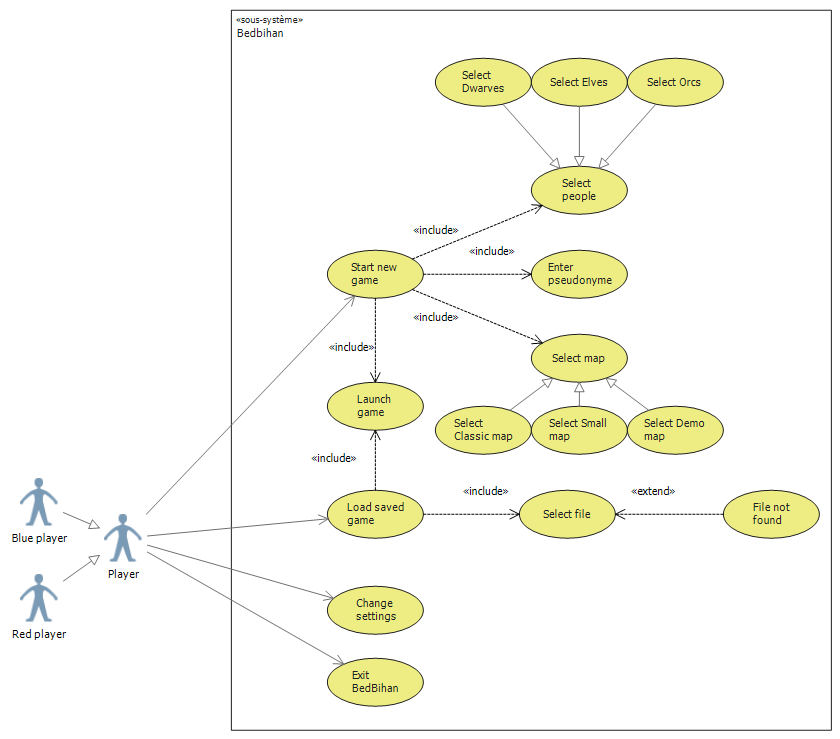
\includegraphics[width=1\textwidth]{figure/cas_utilisation_1.png}
			\end{center}
			\caption{Cas d'utilisation numéro 1}
			\label{fig:use1}
		\end{figure}



	\subsection{le déroulement d'un tour}

		\emph{BedBihan} se joue à tour de rôle. Lors d'un tour le joueur dispose d'un nombre définie d'actions à réaliser. Cela est illusté par le diagramme d'utilisation présenté en FIGURE \ref{fig:use2}.

		\begin{figure}
			\begin{center}
				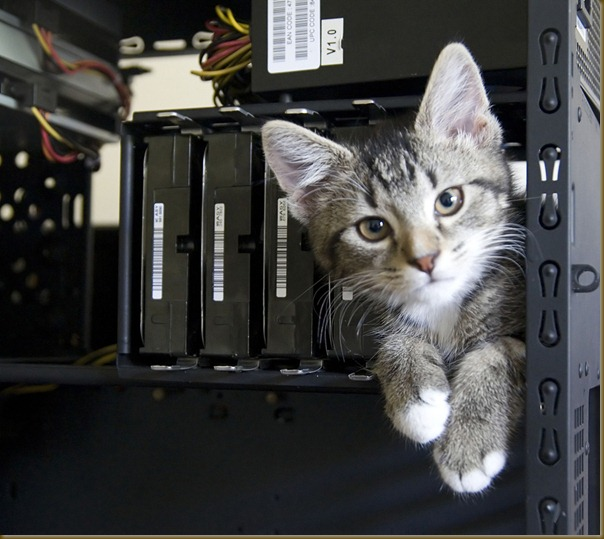
\includegraphics[width=1\textwidth]{figure/cas_utilisation_2.png}
			\end{center}
			\caption{Cas d'utilisation numéro 2}
			\label{fig:use2}
		\end{figure}

	\section{cycle de vie d'une unité}

	Chaque joueur dispose d'un nombre limités d'unités. Chacune de ses unités posséde un certain nombre de point de vie. Lorsque pendant une bataille ce nombre de point de vie est réduit à zéro elle meurt. Elle dispose à chaque tour d'un point de déplacement qu'elle peut utilisé pour ce déplacer ou non. Le déplacement d'une unité sur une casé ocupée par une unité ennemie provoque un combat. Ceci est illustré par le diagramme d'activité en FIGURE \ref{fig:arbre_exemple_1}


	\begin{figure}[h]
	            \centering
	            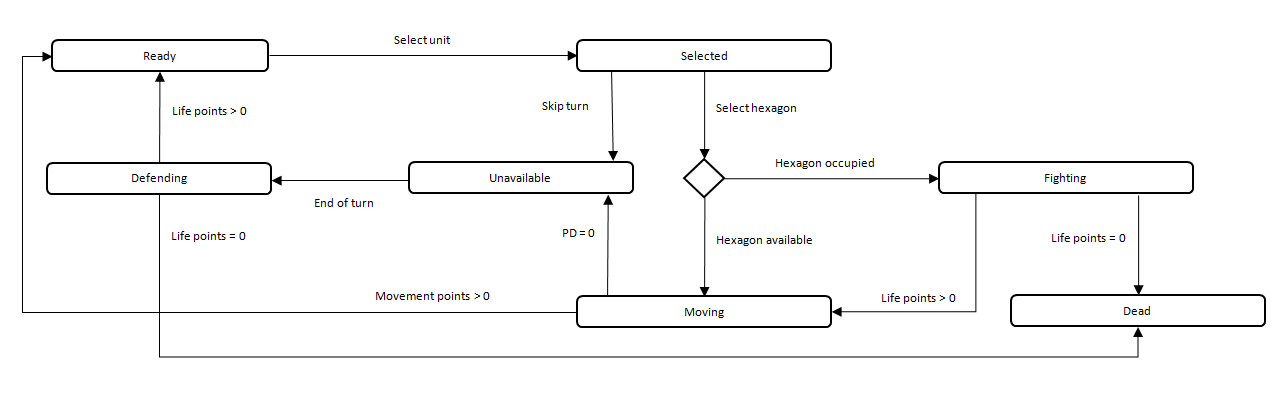
\includegraphics[width=1\textwidth]{figure/unit_life_cycle_state_diagram.png}
	            \caption{Cycle de vie d'une unité.}
	            \label{fig:arbre_exemple_1}
	\end{figure}

		\subsection{le déroulement d'un combat}


		Dans \emph{BedBihan}, quand un joueur souhaite déplacer une unité sur une case occupée par une unité enemie, il provoque un combat. 
